\newsection
\section*{ПРИЛОЖЕНИЕ А \\ Представление графического материала}
\addcontentsline{toc}{section}{ПРИЛОЖЕНИЕ А Представление графического материала}

Графический материал, выполненный на отдельных листах,
изображен на рисунках А.1--А.10.

\renewcommand{\thefigure}{А.\arabic{figure}} % шаблон номера рисунков

\begin{figure}
  \begin{adjustbox}{addcode={\begin{minipage}{\width}}{\caption{%
          Сведения о ВКРБ
      }\end{minipage}},rotate=90,center}
    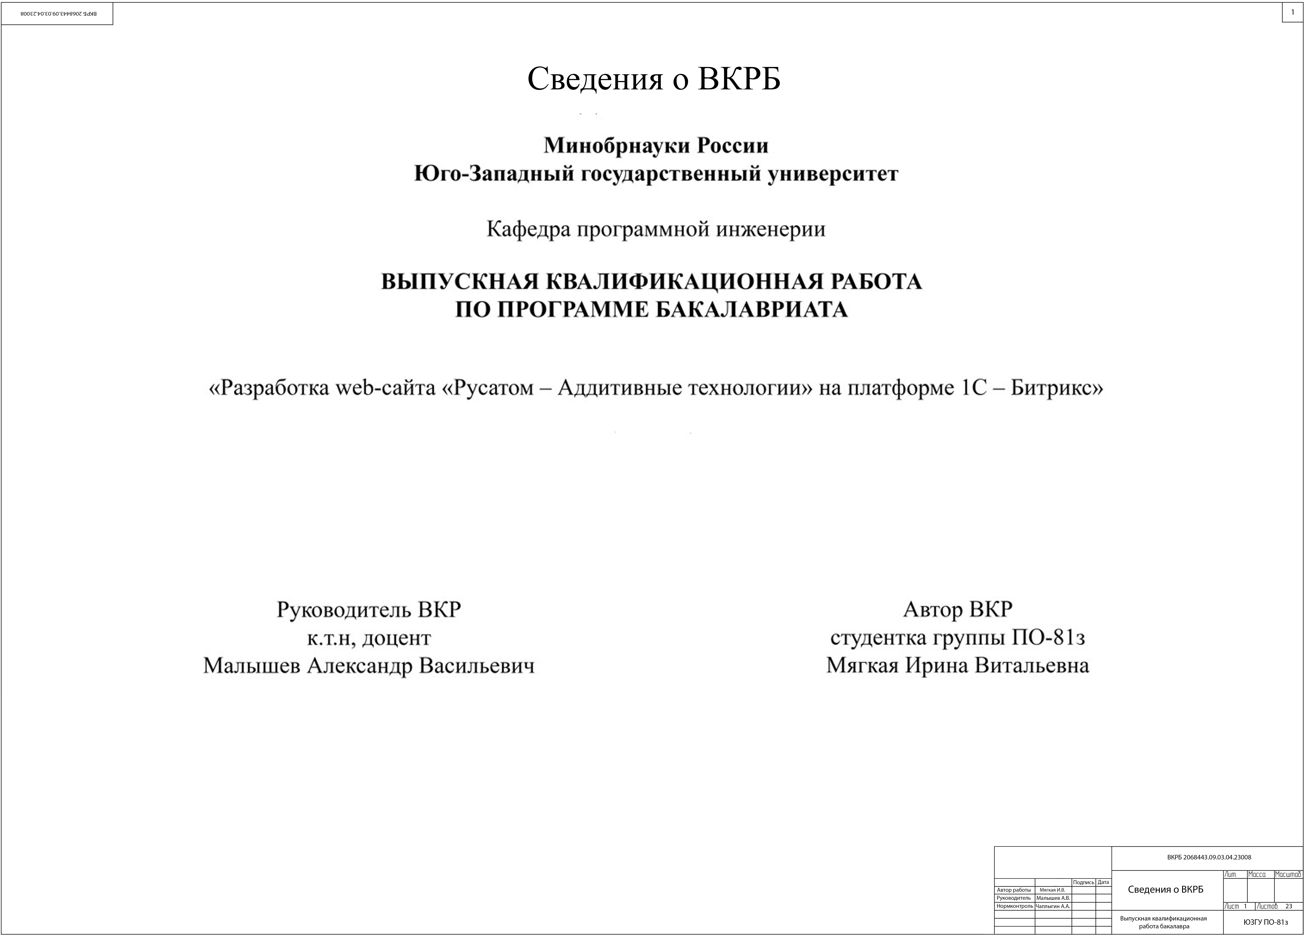
\includegraphics[width=1.3\linewidth]{плакат1.png}
  \end{adjustbox}
  \label{pl1:image}      
\end{figure}

\begin{figure}
  \begin{adjustbox}{addcode={\begin{minipage}{\width}}{\caption{%
          Цель и задачи разработки
      }\end{minipage}},rotate=90,center}
    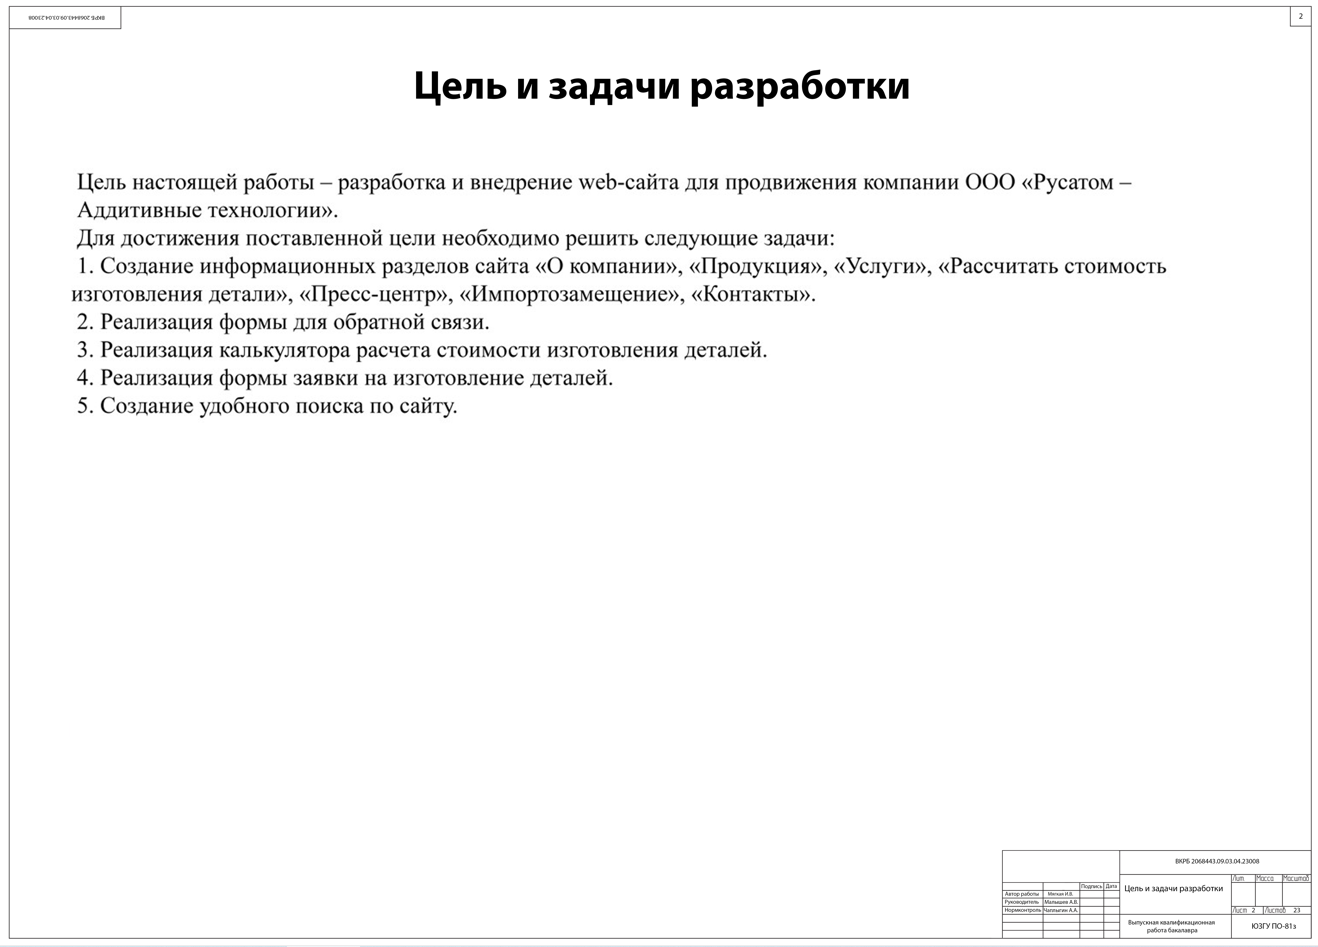
\includegraphics[width=1.3\linewidth]{плакат2.png}
  \end{adjustbox}
  \label{pl2:image}      
\end{figure}

\begin{figure}
  \begin{adjustbox}{addcode={\begin{minipage}{\width}}{\caption{%
          Концептуальная модель сайта
      }\end{minipage}},rotate=90,center}
    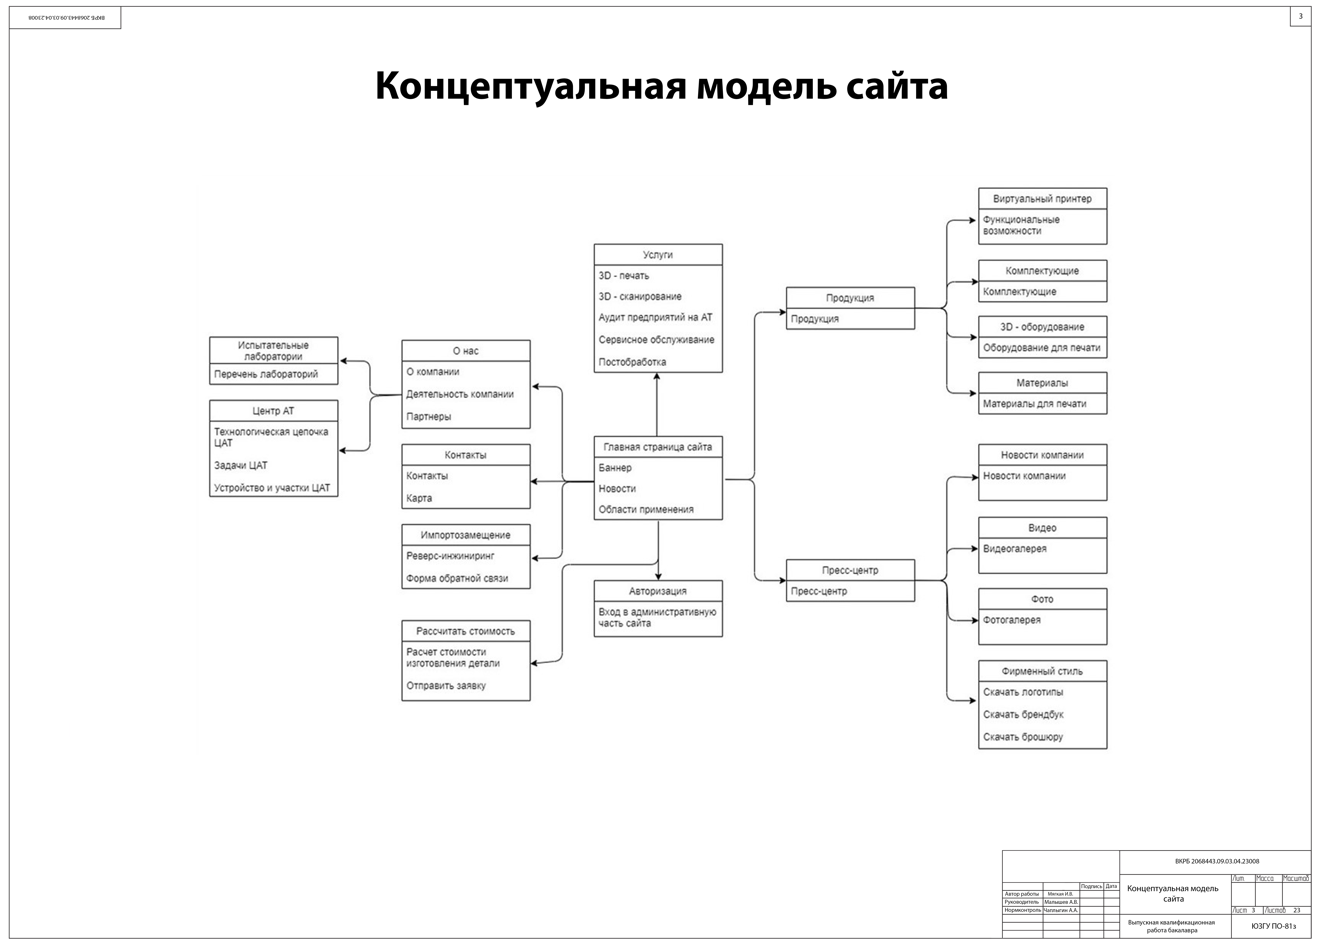
\includegraphics[width=1.3\linewidth]{плакат3.png}
  \end{adjustbox}
  \label{pl3:image}      
\end{figure}
